\addcontentsline{toc}{section}{\textbf{CAPÍTULO III}}
\addcontentsline{toc}{section}{\textbf{MARCO TEÓRICO REFERENCIAL}}

\subsection{Antecedentes}
\subsubsection{Antecedentes internacionales}
\begin{enumerate}[label=\alph*)]

\item Según \textcite{Ning2025}, en su investigación sobre la sumarización personalizada consciente de la intención en textos educativos utilizando Modelos de Lenguaje Grande (LLMs), se encontró que el modelado explícito de la intención del usuario mejora drásticamente la relevancia y exactitud de los resúmenes. Su sistema propuesto logró superar a más de 10 modelos base de referencia, obteniendo ganancias de 6 a 8 puntos en las métricas ROUGE y una mejora de más del 5\% en la consistencia factual medida por la métrica FactCC.

\item Según \textcite{Chen2023}, en su investigación sobre la mejora de la sumarización abstractiva mediante la integración de Grafos de Conocimiento y transformadores de múltiples fuentes, se encontró que el uso de representaciones semánticas estructuradas como guía mitiga la incapacidad intrínseca de los LLMs para verificar la corrección de los hechos. Su modelo MultiBART-GAT demostró un rendimiento superior al generar resúmenes informativos y relevantes, logrando incrementar la puntuación ROUGE-1 a 39.1 y manteniendo un alto nivel de similitud semántica en la evaluación BERTScore.

\item Según \textcite{Jiang2025}, en su investigación sobre el sistema de toma de apuntes colaborativo e inteligente NexaNota, se encontró que la construcción automática de redes de temas mediante grafos de conocimiento impacta positivamente en la eficiencia del aprendizaje. En su estudio, la extracción y representación del conocimiento en el sistema alcanzó una precisión del 97.7\% en la identificación de tópicos principales y una exactitud del 86.7\% al establecer las conexiones semánticas entre dichos tópicos.

\item Según \textcite{Kreijkes2026}, en su investigación sobre los efectos del uso de Modelos de Lenguaje Grande (LLMs) y la toma de apuntes en la comprensión lectora y la memoria, se encontró que combinar la toma de apuntes tradicional con el uso de LLMs tiene efectos positivos significativos en la retención de conocimientos en comparación con el uso exclusivo de la IA. Sus resultados demostraron que el esfuerzo cognitivo involucrado en la estructuración propia de apuntes, apoyado por la IA, mejora las métricas de retención literal y comprensión con un tamaño del efecto estadístico ($d$) de 0.44 y 0.38, respectivamente.

\item Según \textcite{AlvarezPerez2026}, en su investigación desarrollada en México centrada en el \textit{fine-tuning} de modelos \textit{Transformers} para la conversión de textos científicos manuscritos al formato estructurado LaTeX, se encontró que arquitecturas visuales de extremo a extremo, como Nougat y TrOCR, superan ampliamente a los sistemas de OCR convencionales al procesar fórmulas matemáticas. Tras el entrenamiento con un corpus específico, el modelo optimizado demostró una alta capacidad para digitalizar notación espacial compleja, reduciendo la Tasa de Error de Caracteres (CER) hasta un 24.42\% en secuencias manuscritas desafiantes, lo que resulta ser un avance indispensable para la digitalización técnica en ingenierías y un aporte relevante al contexto latinoamericano.

\item Según \textcite{KardanMoghaddam2025}, en su investigación sobre una estructura combinada de transformadores TrOCR y LLMs para la clasificación y extracción de textos manuscritos, se encontró que inyectar las transcripciones de los modelos de visión directamente en un LLM mejora sustancialmente la precisión del procesamiento. Su modelo híbrido (TrOCR-Large acoplado con BART-Large) logró clasificar secuencias de texto con una precisión general (\textit{accuracy}) de 65.29\% y altas puntuaciones F1, demostrando la viabilidad de utilizar \textit{pipelines} de IA en cascada para digitalizar apuntes ruidosos.

\item Según \textcite{Solanki2026}, en su investigación sobre el ecosistema inteligente "NoteGenius", se encontró que la integración de IA generativa para la creación de apuntes y el aprendizaje colaborativo mitiga el problema de la fragmentación de la información académica. El desarrollo de esta plataforma (basada en tecnologías modernas y almacenamiento en la nube) automatiza la generación de resúmenes, conversión de diapositivas y creación de cuestionarios (quizzes), lo cual impacta directamente de forma positiva en la retención de conocimientos y auto-evaluación del estudiante.

\item Según \textcite{Upadhyay2026}, en su estudio sobre una aplicación web integral para el análisis automático de contenido y generación de apuntes a partir de videos de YouTube, se evidenció que la orquestación de APIs de Modelos de Lenguaje Grande (LLMs) con arquitecturas escalables (como React, Express.js y PostgreSQL) optimiza sustancialmente el tiempo de estudio. El sistema logra extraer transcripciones y estructurar apuntes de manera rápida y segura, demostrando la eficacia de los \textit{pipelines} de IA en el procesamiento de contenido multimedia educativo.

\item Según \textcite{Shirkande2025}, en su evaluación del sistema "Noteverse", se identificó que las herramientas tradicionales de gestión de conocimiento adolecen de falta de personalización y de mecanismos de organización inteligente. Su investigación valida que implementar bases de datos en la nube y \textit{frameworks} interactivos como Next.js para lograr una sincronización y coedición en tiempo real es vital para la construcción de ecosistemas colaborativos robustos en la educación superior.
\end{enumerate}

\subsubsection{Antecedentes nacionales}

\begin{enumerate}[label=\alph*)]
\item Según \textcite{TarazonaCruz2024}, en su investigación sobre el reconocimiento de texto en manuscritos históricos peruanos utilizando modelos mixtos, se encontró que el uso de modelos de reconocimiento de imágenes preentrenados mediante la plataforma de código abierto OCR4all es viable para digitalizar documentos manuscritos en español. Tras entrenar tres modelos con el conjunto de datos SPA-Sentences (aproximadamente 13,000 oraciones), su sistema alcanzó una Tasa de Error de Caracteres (CER) promedio de 4.11\% en el conjunto de validación, y al aplicarlo sobre manuscritos históricos peruanos de la Biblioteca Nacional del Perú obtuvo una tasa de error promedio de 9.39\%, demostrando la utilidad de estas arquitecturas para el contexto local pese a la variabilidad caligráfica y el deterioro del papel.
\end{enumerate}

\subsection{Marco teórico}

\subsubsection{Inteligencia Artificial Generativa y Arquitectura RAG}

La Inteligencia Artificial Generativa, particularmente impulsada por Modelos de Lenguaje 
Grande (LLMs) como GPT-3.5 o LLaMA 3, ha revolucionado las tareas de procesamiento de 
lenguaje natural al habilitar la sumarización abstractiva de textos con alta coherencia 
\parencite{Saxena2025}. No obstante, estos modelos probabilísticos carecen de mecanismos 
intrínsecos para verificar la veracidad de la información que generan, lo que con 
frecuencia deriva en ``alucinaciones'': información plausible pero fácticamente incorrecta 
\parencite{Chen2023}.

Para mitigar este problema, surge la arquitectura de Generación Aumentada por Recuperación 
(RAG). En lugar de depender exclusivamente de los pesos preentrenados del modelo, RAG 
restringe el espacio de inferencia recuperando primero los fragmentos de texto más 
relevantes desde un corpus local y proporcionándolos como contexto estricto al LLM 
\textcite{Kannammal2024}. El \textit{pipeline} RAG clásico comprende tres etapas: 
indexación del corpus mediante \textit{embeddings} vectoriales, recuperación semántica 
por similitud de coseno, y generación condicionada al contexto recuperado 
\parencite{GaoRAGSurvey2024}. Al acoplar RAG con validadores factuales, la tasa de 
alucinaciones se minimiza de forma crítica \textcite{Ning2025}, lo que resulta 
especialmente relevante para sistemas educativos donde la exactitud del contenido generado 
es indispensable. La evolución más reciente ha dado lugar a variantes como GraphRAG, que 
integra grafos de conocimiento en el proceso de recuperación para capturar relaciones 
estructuradas entre conceptos, superando las limitaciones de la recuperación puramente 
vectorial \parencite{KleselWittmannRAG2025}.

\begin{figure}[H]
    \centering
    \begin{tikzpicture}[
        node distance=1.5cm and 1.8cm,
        box/.style={draw, rectangle, rounded corners, fill=blue!10, text width=2.5cm, align=center, minimum height=1.2cm, font=\small},
        cloud/.style={draw, ellipse, fill=yellow!15, text width=2.2cm, align=center, minimum height=1.2cm, font=\small},
        arrow/.style={-Stealth, thick}
    ]
        % Row 1
        \node[box] (query) {Pregunta del Usuario};
        \node[box, right=of query] (embed) {Modelo de Embeddings};
        \node[box, right=of embed] (search) {Búsqueda por Similitud};
        
        % Row 2
        \node[cloud, below=of search] (db) {Base de Datos Vectorial};
        
        % Row 3
        \node[box, below=of embed] (context) {Contexto Recuperado};
        \node[box, below=of query] (llm) {LLM (Generador)};
        \node[box, left=of llm] (response) {Respuesta Final};
        
        % Arrows
        \draw[arrow] (query) -- (embed);
        \draw[arrow] (embed) -- (search);
        \draw[arrow] (search) -- (db);
        \draw[arrow] (db) -- (context);
        \draw[arrow] (context) -- (llm);
        \draw[arrow] (llm) -- (response);
        \draw[arrow] (query) -- (llm);
    \end{tikzpicture}
    \caption{Arquitectura general del sistema de Generación Aumentada por Recuperación (RAG).}
    \label{fig:rag_architecture}
\end{figure}

\subsubsection{Arquitectura Transformer y Mecanismo de Atención}

El fundamento técnico de los LLMs y de los modelos de visión empleados en el presente 
proyecto reside en la arquitectura Transformer, introducida por \textcite{Vaswani2017} 
en el trabajo seminal ``Attention is All You Need''. A diferencia de las arquitecturas 
recurrentes (RNN/LSTM) que procesan secuencias de forma estrictamente secuencial, el 
Transformer opera mediante un mecanismo de \textit{auto-atención} (\textit{Self-Attention}) 
que calcula, en paralelo, la relevancia relativa de cada posición de la secuencia respecto 
a todas las demás. Formalmente, la atención escalada de producto punto se define como:

\begin{equation}
    \text{Attention}(Q, K, V) = \text{softmax}\!\left(\frac{QK^\top}{\sqrt{d_k}}\right)V
\end{equation}

donde $Q$, $K$ y $V$ representan las matrices de \textit{queries}, \textit{keys} y 
\textit{values} proyectadas, y $d_k$ es la dimensión de las \textit{keys}, cuya raíz 
cuadrada actúa como factor de escala para estabilizar los gradientes 
\parencite{Vaswani2017}. La extensión multi-cabeza (\textit{Multi-Head Attention}) 
ejecuta múltiples operaciones de atención en paralelo sobre distintos subespacios de 
representación, permitiendo al modelo capturar simultáneamente dependencias sintácticas, 
semánticas y de largo alcance en el texto \parencite{Vaswani2017}.

\begin{figure}[H]
    \centering
    \begin{tikzpicture}[
        node distance=1cm and 1.5cm,
        op/.style={draw, circle, fill=yellow!20, minimum size=0.8cm, font=\small},
        val/.style={draw, rectangle, fill=green!10, minimum width=1.5cm, minimum height=0.6cm, font=\small},
        arrow/.style={-Stealth, thick}
    ]
        % Nodes
        \node[val] (q) {Queries ($Q$)};
        \node[val, right=of q] (k) {Keys ($K$)};
        \node[val, right=of k] (v) {Values ($V$)};
        
        \node[op, below=of k] (matmul1) {$\otimes$};
        \node[op, below=of matmul1] (scale) {$\div \sqrt{d_k}$};
        \node[op, below=of scale] (softmax) {Softmax};
        \node[op, below=of softmax, xshift=1.2cm] (matmul2) {$\otimes$};
        \node[val, below=of matmul2] (out) {Atención ($Attention$)};
        
        % Connections
        \draw[arrow] (q) |- (matmul1);
        \draw[arrow] (k) -- (matmul1);
        \draw[arrow] (matmul1) -- (scale);
        \draw[arrow] (scale) -- (softmax);
        \draw[arrow] (softmax) |- (matmul2);
        \draw[arrow] (v) |- (matmul2);
        \draw[arrow] (matmul2) -- (out);
    \end{tikzpicture}
    \caption{Mecanismo de auto-atención escalada por producto punto (Scaled Dot-Product Attention).}
    \label{fig:self_attention_mechanism}
\end{figure}

Esta arquitectura fue posteriormente adaptada al dominio de la visión por computadora 
mediante el Vision Transformer (ViT), que divide una imagen en parches (\textit{patches}) 
de tamaño fijo, los proyecta linealmente y los procesa como una secuencia de tokens, 
habilitando la captura de dependencias globales entre regiones de la imagen 
\parencite{LiTrOCR2023}. Es precisamente esta sinergia entre un codificador de visión 
basado en ViT y un decodificador de lenguaje autorregresivo la que subyace al modelo 
TrOCR, pilar tecnológico del módulo de transcripción de SynapTome.

\subsubsection{Reconocimiento de Texto Manuscrito (HTR), TrOCR y Fórmulas Matemáticas}

El Reconocimiento Óptico de Caracteres (OCR) tradicional se fundamenta en múltiples 
módulos independientes: preprocesamiento, segmentación, extracción de características 
mediante CNN y postprocesamiento, lo que genera una alta propagación de errores y una 
notable ineficiencia frente a caligrafía compleja \parencite{Zhang2026}. Los sistemas 
CNN-RNN presentan además limitaciones al procesar texto manuscrito con alta variabilidad 
caligráfica, pues su campo receptivo local impide capturar dependencias de largo alcance 
entre caracteres \parencite{LiTrOCR2023}.

En contraparte, TrOCR unifica estas tareas en una arquitectura única de extremo a extremo. 
Emplea un codificador de visión preentrenado (BEiT o DeiT) para extraer características 
visuales de la imagen en parches, y un decodificador de lenguaje (RoBERTa) que genera 
el texto de manera autorregresiva \textcite{LiTrOCR2023}. El modelo 
TrOCR\textsubscript{LARGE} alcanza una Tasa de Error de Caracteres (CER) de apenas 
2,89\% en el \textit{benchmark} IAM, superando a todos los modelos CNN-RNN previos 
\parencite{SharmaTrOCR2025}.

Una dimensión especialmente crítica para SynapTome es el Reconocimiento de Expresiones 
Matemáticas Manuscritas (HMER, por sus siglas en inglés). A diferencia del texto corriente, 
las fórmulas matemáticas presentan una estructura bidimensional compleja: superíndices, 
subíndices, fracciones, integrales y símbolos especiales cuya disposición espacial es 
parte integrante de su significado. Los modelos encoder-decoder basados en Transformers, 
como UniMERNet, abordan esta complejidad mediante la generación directa de código \LaTeX{} 
a partir de la imagen de la fórmula, logrando reconocer con alta precisión tanto 
expresiones impresas como manuscritas en escenarios reales \parencite{AlvarezPerez2026}. 
El conjunto de datos MathWriting, que provee anotaciones \LaTeX{} para fórmulas 
manuscritas en línea (\textit{online}) y fuera de línea (\textit{offline}), constituye 
actualmente el referente de evaluación para estos modelos \parencite{AlvarezPerez2026}. 
En el contexto peruano, arquitecturas preentrenadas de esta familia han demostrado ser 
viables incluso para manuscritos con alta variabilidad caligráfica \parencite{TarazonaCruz2024}.

\begin{figure}[H]
    \centering
    \begin{tikzpicture}[
        node distance=2.2cm,
        stage/.style={draw, rectangle, fill=orange!15, text width=3cm, align=center, minimum height=1cm, rounded corners, font=\small},
        arrow/.style={-Stealth, thick}
    ]
        % Nodes
        \node[stage] (img) {Imagen de Apunte (Manuscrito)};
        \node[stage, right=of img] (enc) {Codificador de Visión (ViT)};
        \node[stage, right=of enc] (dec) {Decodificador de Texto (RoBERTa)};
        \node[stage, below=of dec] (latex) {Código \LaTeX{} estructurado};
        
        % Connections
        \draw[arrow] (img) -- (enc);
        \draw[arrow] (enc) -- node[above, font=\scriptsize] {Embeddings visuales} (dec);
        \draw[arrow] (dec) -- (latex);
    \end{tikzpicture}
    \caption{Flujo de procesamiento híbrido de visión y lenguaje del modelo TrOCR.}
    \label{fig:trocr_flow_diagram}
\end{figure}

\subsubsection{\textit{Vector Embeddings} y Bases de Datos Vectoriales}

Los \textit{embeddings} vectoriales son representaciones numéricas de alta dimensión que 
codifican el significado semántico de fragmentos de texto, imágenes u otros tipos de 
datos. La propiedad fundamental de estos vectores es que la proximidad geométrica en 
el espacio vectorial refleja similitud semántica: fragmentos con significado afín 
producen vectores cercanos, independientemente de si comparten vocabulario exacto 
\parencite{GaoRAGSurvey2024}. Este principio constituye la base técnica de la 
recuperación semántica en los sistemas RAG: al codificar tanto los fragmentos del 
corpus como la consulta del usuario en el mismo espacio vectorial, es posible recuperar 
los $k$ fragmentos más relevantes mediante una búsqueda de vecinos más cercanos 
(\textit{k-NN search}).

Para la persistencia y consulta eficiente de estos vectores en el contexto de SynapTome, 
la extensión \texttt{pgvector} para PostgreSQL representa la solución arquitectónica 
óptima. Esta extensión permite almacenar vectores de alta dimensión directamente en 
tablas relacionales y ejecutar búsquedas de similitud mediante los operadores de 
distancia coseno, euclídea o producto punto, combinando las capacidades de búsqueda 
semántica con las garantías ACID y las operaciones relacionales estándar de SQL 
\parencite{Afian2025}. La indexación mediante estructuras HNSW 
(\textit{Hierarchical Navigable Small World}) permite escalar estas búsquedas a 
millones de vectores con latencias de consulta inferiores a 10 ms, manteniendo una 
alta tasa de recuperación (\textit{recall}) \parencite{Upadhyay2026}. Esta arquitectura 
unificada — datos relacionales y vectores en una sola base de datos — simplifica 
significativamente la infraestructura del sistema y elimina la necesidad de sincronizar 
datos entre una base de datos relacional y un almacén vectorial independiente.

\begin{figure}[H]
    \centering
    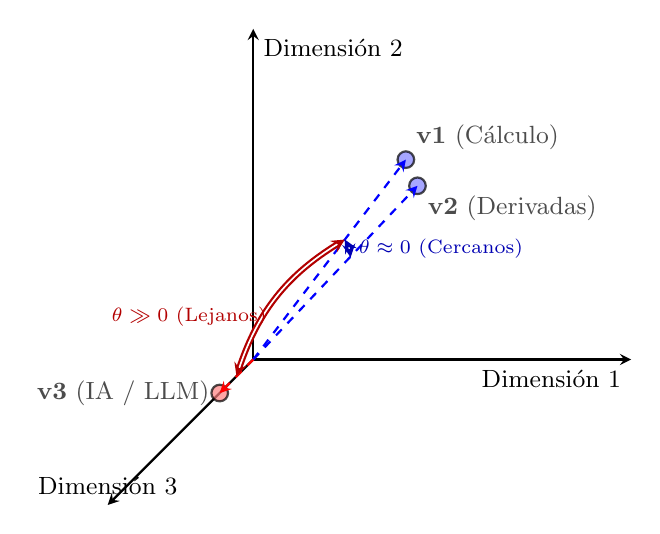
\begin{tikzpicture}[scale=1.2, >=stealth, thick]
        % Coordinate axis
        \draw[->] (0,0,0) -- (4,0,0) node[anchor=north east, font=\small]{Dimensión 1};
        \draw[->] (0,0,0) -- (0,3.5,0) node[anchor=north west, font=\small]{Dimensión 2};
        \draw[->] (0,0,0) -- (0,0,4) node[anchor=south, font=\small]{Dimensión 3};
        
        % Vector points
        \draw[fill=blue!50, opacity=0.7] (2,2.5,1) circle (2.5pt) node[anchor=south west, font=\small] {\textbf{v1} (Cálculo)};
        \draw[fill=blue!50, opacity=0.7] (2.2,2.3,1.2) circle (2.5pt) node[anchor=north west, font=\small] {\textbf{v2} (Derivadas)};
        \draw[fill=red!50, opacity=0.7] (0.8,0.8,3) circle (2.5pt) node[anchor=east, font=\small] {\textbf{v3} (IA / LLM)};
        
        % Cosine similarity arcs/lines
        \draw[dashed, ->, blue] (0,0,0) -- (2,2.5,1);
        \draw[dashed, ->, blue] (0,0,0) -- (2.2,2.3,1.2);
        \draw[dashed, ->, red] (0,0,0) -- (0.8,0.8,3);
        
        \draw[double, <->, blue!70!black] (1.2,1.5,0.6) to[bend left=10] node[midway, right, font=\scriptsize] {$\theta \approx 0$ (Cercanos)} (1.3,1.35,0.7);
        \draw[double, <->, red!70!black] (1.2,1.5,0.6) to[bend right=20] node[midway, below left, font=\scriptsize] {$\theta \gg 0$ (Lejanos)} (0.4,0.4,1.5);
    \end{tikzpicture}
    \caption{Similitud de coseno entre vectores en un espacio de embeddings multidimensional.}
    \label{fig:cosine_similarity_embeddings}
\end{figure}

\subsubsection{Grafos de Conocimiento}

Los Grafos de Conocimiento son estructuras matemáticas que representan la información 
como una red semántica dirigida, conformada por nodos (entidades o tópicos) y aristas 
(relaciones). Esta topología permite capturar el contexto global y las relaciones 
transversales dentro de un corpus documental, sirviendo como esqueleto para la 
extracción de características y el aprendizaje representacional \textcite{Chen2023}. 
Una revisión sistemática reciente identifica que su principal aporte en educación 
reside en la capacidad de modelar la progresión del conocimiento del estudiante a lo 
largo del tiempo, conectando conceptos de distintas asignaturas y niveles cognitivos 
\parencite{AbuSalih2024}. En este sentido, permiten representar el estado de aprendizaje 
de cada alumno como una red dinámica de nodos de competencia, facilitando la 
personalización de rutas de estudio y la identificación de brechas conceptuales 
\parencite{SoumyaKrishnamoorthy2025}.

En el contexto de sistemas de gestión del aprendizaje, estos mapas de tópicos 
transforman el contenido aislado en recursos enlazados, impulsando la 
``Inteligencia Colectiva'' \parencite{Obionwu2022}. La integración de grafos de 
conocimiento con arquitecturas RAG —denominada GraphRAG— representa el estado del 
arte en recuperación semántica educativa: al estructurar el corpus de apuntes como 
un grafo, el sistema puede recorrer relaciones semánticas para recuperar fragmentos 
contextualmente relevantes que la búsqueda vectorial clásica no identificaría 
\parencite{EduGraphRAG2025}. Para su implementación en el \textit{backend}, 
PostgreSQL con \texttt{pgvector} garantiza la integridad, el indexado veloz y el 
almacenamiento seguro de los metadatos y vectores de las entidades semánticas 
\parencite{Afian2025, Upadhyay2026}.

\begin{figure}[H]
    \centering
    \begin{tikzpicture}[
        node distance=2cm,
        node/.style={draw, circle, fill=purple!15, text width=1.8cm, align=center, minimum size=1.8cm, font=\small},
        arrow/.style={-Stealth, thick}
    ]
        % Nodes
        \node[node] (std) {Estudiante};
        \node[node, right=of std, xshift=1cm] (deriv) {Tema: Derivadas};
        \node[node, below=of deriv] (lim) {Tema: Límites};
        
        % Connections
        \draw[arrow] (std) -- node[above, font=\scriptsize] {estudia} (deriv);
        \draw[arrow] (deriv) -- node[right, font=\scriptsize] {requiere} (lim);
        \draw[arrow] (std) -- node[below left, font=\scriptsize] {revisa} (lim);
    \end{tikzpicture}
    \caption{Grafo relacional de conocimiento representando la progresión del estudiante.}
    \label{fig:educational_knowledge_graph}
\end{figure}

\subsubsection{Generación Automática de Evaluaciones Adaptativas}

La generación automática de cuestionarios a partir del contenido de apuntes constituye 
una de las aplicaciones más directas de los LLMs en educación. Los sistemas basados en 
IA son capaces de producir ítems alineados con la Taxonomía de Bloom —desde preguntas 
de recordación hasta ítems de evaluación y creación— a partir de fragmentos de texto, 
reduciendo significativamente la carga docente \parencite{QuerIA2025}. Herramientas 
como QuizWiz demuestran que los LLMs integrados en plataformas educativas pueden 
generar cuestionarios personalizados y adaptativos en tiempo real, ajustando la 
dificultad al nivel de dominio actual del estudiante \parencite{QuizWiz2024}.

Los grafos de conocimiento desempeñan un rol instrumental en esta dinámica: al 
estructurar los apuntes como una red de conceptos relacionados, el sistema selecciona 
de forma dirigida los nodos temáticos sobre los cuales generar preguntas, garantizando 
cobertura curricular equilibrada y evitando redundancia \parencite{PersonalizedLearningKG2026}. 
Esta sinergia entre grafos de conocimiento y generación automática de evaluaciones 
constituye el núcleo de la variable independiente 3 del presente proyecto.

\subsubsection{Aprendizaje Activo y Recuperación Espaciada (\textit{Spaced Repetition})}

La Teoría de la Recuperación Espaciada (\textit{Spaced Repetition}) se fundamenta en 
la curva del olvido de Ebbinghaus, que describe cómo la tasa de retención decae 
exponencialmente con el tiempo en ausencia de revisiones. La estrategia consiste en 
programar las revisiones de un concepto justo antes del momento en que será olvidado, 
maximizando la consolidación en la memoria a largo plazo mediante el denominado 
\textit{efecto de espaciado} \parencite{Huang2025}. La práctica de recuperación activa 
(\textit{Active Recall}) complementa esta estrategia: en lugar de releer pasivamente 
el material, el estudiante intenta recordar activamente la información, lo que fortalece 
las trazas mnémicas de forma significativamente más efectiva que la revisión pasiva; 
estudios recientes demuestran que los estudiantes que practican recuperación activa 
superan en más de un 50\% en pruebas diferidas a quienes solo releen el material 
\parencite{Huang2025}.

Los sistemas de repetición espaciada modernos han evolucionado desde modelos de 
intervalo fijo —como el sistema Leitner— hacia algoritmos adaptativos basados en 
datos, como FSRS5 (\textit{Free Spaced Repetition Scheduler}), que estima dinámicamente 
el intervalo óptimo de revisión para cada ítem según el historial de respuestas del 
estudiante \parencite{SpacedRepetitionLLM2025}. La integración de LLMs en estos sistemas 
permite generar automáticamente las tarjetas de estudio (\textit{flashcards}) a partir 
del contenido de los apuntes digitalizados, cerrando el ciclo entre transcripción, 
estructuración y refuerzo del aprendizaje \parencite{SpacedRepetitionLLM2025}. En el 
contexto de SynapTome, este módulo se articula directamente con el motor de grafos de 
conocimiento: los nodos con menor frecuencia de revisión o menor puntuación de dominio 
activan automáticamente la generación de nuevas instancias de práctica de recuperación.

\begin{figure}[H]
    \centering
    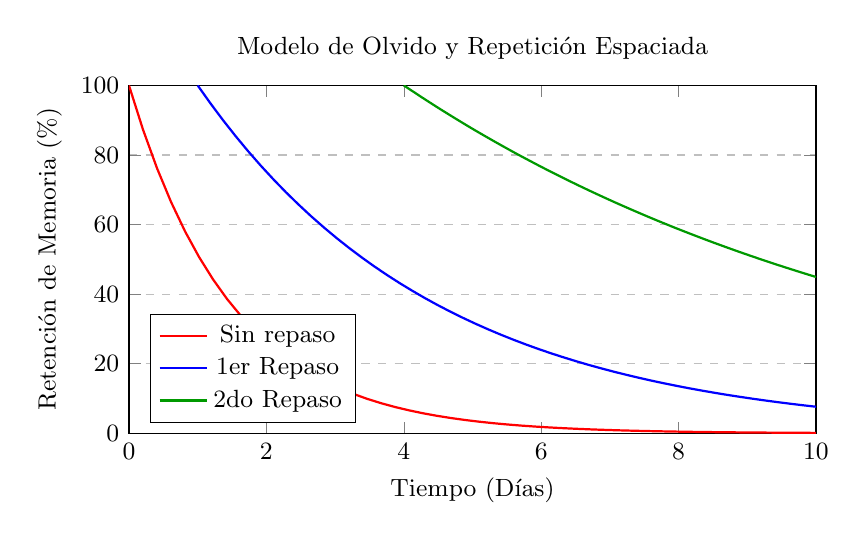
\begin{tikzpicture}
        \begin{axis}[
            title={Modelo de Olvido y Repetición Espaciada},
            xlabel={Tiempo (Días)},
            ylabel={Retención de Memoria (\%)},
            xmin=0, xmax=10,
            ymin=0, ymax=100,
            xtick={0,2,4,6,8,10},
            ytick={0,20,40,60,80,100},
            legend pos=south west,
            ymajorgrids=true,
            grid style=dashed,
            width=0.85\textwidth,
            height=6cm,
            font=\small
        ]
            % Curve 1: initial learning (day 0)
            \addplot[color=red, domain=0:10, samples=50, thick] {100*exp(-x/1.5)};
            \addlegendentry{Sin repaso}
            
            % Curve 2: review at day 1
            \addplot[color=blue, domain=1:10, samples=50, thick] {100*exp(-(x-1)/3.5)};
            \addlegendentry{1er Repaso}
            
            % Curve 3: review at day 4
            \addplot[color=green!60!black, domain=4:10, samples=50, thick] {100*exp(-(x-4)/7.5)};
            \addlegendentry{2do Repaso}
        \end{axis}
    \end{tikzpicture}
    \caption{Curva del olvido de Ebbinghaus y el impacto de los repasos programados.}
    \label{fig:forgetting_curve_rep_esp}
\end{figure}

\subsubsection{Aprendizaje Colaborativo Mediado por Tecnología}

El aprendizaje colaborativo, entendido como el proceso mediante el cual los estudiantes 
construyen conocimiento de forma conjunta a través del intercambio de recursos, ha sido 
ampliamente validado como estrategia que mejora la retención y el desempeño académico 
\parencite{Kasirye2023}. Una revisión sistemática de 148 artículos publicados entre 
2021 y 2024 concluye que las herramientas de IA mejoran la personalización, la 
comunicación entre pares y el andamiaje del rendimiento, al tiempo que promueven 
entornos colaborativos mediante soporte de aprendizaje cooperativo 
\parencite{MsambwaAI2025}. Sin embargo, la evidencia también advierte sobre una tensión 
emergente: el exceso de asistencia de IA en tareas de toma de notas puede reducir el 
compromiso cognitivo activo del estudiante \parencite{AINoteTakingCognition2025}, lo 
que sugiere que SynapTome debe calibrar el nivel de automatización para preservar el 
procesamiento profundo de la información.

\subsubsection{Carga Cognitiva y Medición con NASA-TLX}

La Teoría de la Carga Cognitiva postula que la memoria de trabajo humana posee una 
capacidad limitada para procesar información simultáneamente, y que el diseño de 
entornos de aprendizaje debe minimizar la carga extrínseca para maximizar los recursos 
cognitivos disponibles \parencite{HartStaveland1988}. Para la cuantificación objetiva 
de esta carga, el instrumento NASA Task Load Index (NASA-TLX) constituye el estándar 
de referencia más ampliamente adoptado. Evalúa seis dimensiones: Demanda Mental, 
Demanda Física, Demanda Temporal, Rendimiento, Esfuerzo y Frustración, obteniendo 
un índice global ponderado \parencite{HartStaveland1988}. Su validez ha sido 
reconfirmada recientemente en contextos de interacción humano-computadora 
\parencite{NASATLXReviewHCI2025}. En estudios con estudiantes universitarios, la 
Demanda Temporal y la Demanda Mental emergen como las dimensiones de mayor puntuación, 
con correlaciones significativas entre ambas ($\rho = 0.58$, $p < 0.001$), subrayando 
la relevancia de diseñar sistemas que reduzcan simultáneamente la presión temporal y 
el esfuerzo mental \parencite{Cahyadi2026}.

\subsubsection{Privacidad y Seguridad de Datos Estudiantiles en Plataformas IA}

El despliegue de plataformas educativas potenciadas por IA implica la recopilación y 
procesamiento de datos estudiantiles altamente sensibles: registros académicos, 
patrones de comportamiento, historial de consultas y contenido de apuntes personales. 
La gestión ética y segura de estos datos es un imperativo técnico y legal que condiciona 
el diseño arquitectónico de SynapTome \parencite{XAIEducation2024}. En el ámbito 
normativo internacional, dos marcos regulatorios delimitan las obligaciones de las 
plataformas educativas: la Ley de Privacidad y Derechos Educativos de la Familia 
(FERPA, por sus siglas en inglés), vigente en contextos anglosajones, y el Reglamento 
General de Protección de Datos (GDPR) de la Unión Europea, cuyo alcance extraterritorial 
puede afectar a cualquier plataforma que procese datos de ciudadanos europeos 
\parencite{XAIEducation2024}. Ambos marcos exigen el principio de \textit{minimización 
de datos} —recopilar únicamente los datos estrictamente necesarios—, el consentimiento 
informado, y la implementación de salvaguardas técnicas como cifrado en reposo y en 
tránsito, control de acceso basado en roles (RBAC) y registros de auditoría.

Adicionalmente, la Ley de Inteligencia Artificial de la Unión Europea (EU AI Act) 
clasifica los sistemas de IA utilizados en educación como sistemas de ``alto riesgo'', 
lo que impone obligaciones adicionales de transparencia, explicabilidad y evaluación 
de impacto sobre la privacidad (DPIA) antes de su despliegue \parencite{XAIEducation2024}. 
En el diseño de SynapTome, estas consideraciones se traducen en la adopción de 
Arquitectura Limpia con separación estricta entre la capa de datos y los servicios de 
IA, el cifrado de los \textit{embeddings} vectoriales almacenados en PostgreSQL, y la 
implementación de políticas de retención de datos que permitan la eliminación completa 
del historial de un estudiante a solicitud expresa.

\subsubsection{Arquitectura Limpia (\textit{Clean Architecture})}

La Arquitectura Limpia es un patrón de diseño de software que promueve la separación 
estricta de responsabilidades mediante un sistema de capas concéntricas, aislando la 
lógica de negocio y las reglas del dominio de los \textit{frameworks}, interfaces de 
usuario o bases de datos \textcite{Martin2017}. Su principio central, la Regla de 
Dependencia, establece que los módulos de alto nivel no deben depender de los de bajo 
nivel, sino que ambos deben depender de abstracciones \parencite{Martin2017}.

En el desarrollo de plataformas educativas integrales, mantener un \textit{backend} 
escalable y modular bajo este enfoque resulta indispensable para soportar 
\textit{pipelines} intensivos de IA \textcite{Upadhyay2026, Solanki2026}. Su 
aplicación en ecosistemas basados en C\# y ASP.NET Core permite construir APIs 
RESTful robustas donde los controladores son totalmente independientes de los 
servicios de infraestructura como PostgreSQL o los motores de LLM, asegurando que 
la integración de nuevas tecnologías de IA no afecte el núcleo lógico del sistema 
\parencite{Afian2025}.

\begin{figure}[H]
    \centering
    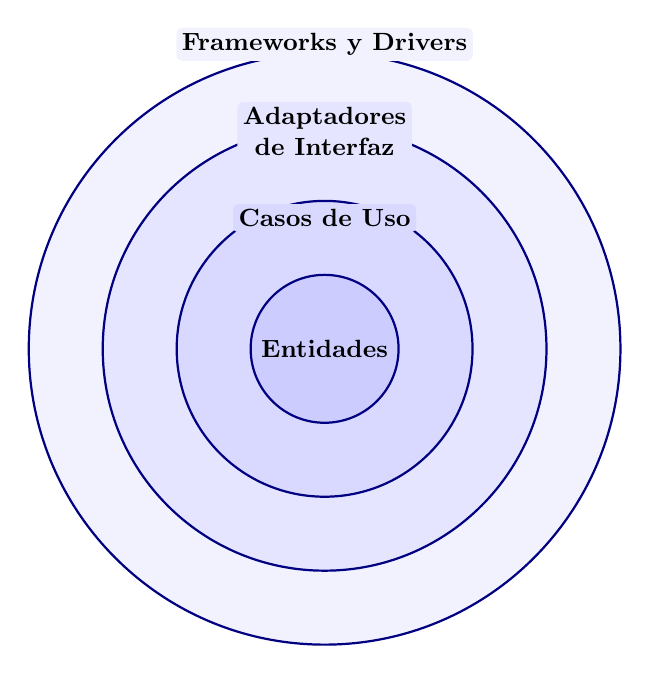
\begin{tikzpicture}[scale=0.85, font=\small]
        % Concentric circles
        \draw[fill=blue!5, draw=blue!50!black, thick] (0,0) circle (4.42cm);
        \draw[fill=blue!10, draw=blue!50!black, thick] (0,0) circle (3.315cm);
        \draw[fill=blue!15, draw=blue!50!black, thick] (0,0) circle (2.21cm);
        \draw[fill=blue!20, draw=blue!50!black, thick] (0,0) circle (1.105cm);
        
        % Labels
        \node at (0,0) [align=center] {\textbf{Entidades}};
        \node at (0,1.95) [align=center, fill=blue!15, inner sep=2pt, rounded corners=2pt] {\textbf{Casos de Uso}};
        \node at (0,3.25) [align=center, fill=blue!10, inner sep=2pt, rounded corners=2pt] {\textbf{Adaptadores}\\\textbf{de Interfaz}};
        \node at (0,4.55) [align=center, fill=blue!5, inner sep=2pt, rounded corners=2pt] {\textbf{Frameworks y Drivers}};
    \end{tikzpicture}
    \caption{Capas concéntricas de dependencias bajo el diseño de Arquitectura Limpia.}
    \label{fig:clean_architecture_layers}
\end{figure}

% ================== MARCO CONCEPTUAL ==================
\subsection{Marco conceptual}

\begin{enumerate}[label=\alph*)]
  \item \textbf{LLM (Large Language Model).} Modelo de inteligencia artificial basado en redes neuronales profundas, típicamente sobre la arquitectura Transformer, entrenado con cantidades masivas de datos para comprender, procesar y generar lenguaje natural de forma coherente \parencite{Vaswani2017, KardanMoghaddam2025}.

  \item \textbf{RAG (Retrieval-Augmented Generation).} Arquitectura que combina la recuperación de fragmentos de información relevantes desde una base de conocimiento externa con la generación de texto de un LLM, utilizada para reducir las alucinaciones y anclar las respuestas a un contexto verificable \parencite{Kannammal2024}.

  \item \textbf{TrOCR (Transformer-based Optical Character Recognition).} Arquitectura de extremo a extremo para el reconocimiento de texto, compuesta por un codificador de visión (por ejemplo, DeiT o BEiT) y un decodificador de lenguaje (por ejemplo, RoBERTa), capaz de transcribir imágenes de texto manuscrito o impreso de manera autorregresiva \parencite{Zhang2026}.

  \item \textbf{Grafo de Conocimiento (Knowledge Graph).} Estructura de datos que representa información como una red semántica dirigida compuesta por nodos (entidades o tópicos) y aristas (relaciones), utilizada para capturar el contexto global y las conexiones entre los conceptos de un corpus \parencite{Chen2023}.

  \item \textbf{Topic Maps (Mapas de Tópicos).} Estándar de representación del conocimiento que define un modelo abstracto para estructurar semánticamente redes de información y enlaces, facilitando el descubrimiento y la conexión de conceptos \parencite{Obionwu2022}.

  \item \textbf{CER y WER (Character/Word Error Rate).} Métricas estándar para evaluar sistemas de reconocimiento de texto, que calculan el porcentaje de caracteres o palabras incorrectamente reconocidos respecto al total del texto de referencia; valores más bajos indican mayor precisión del modelo \parencite{AlHitawi2026}.

  \item \textbf{ROUGE y BERTScore.} Métricas utilizadas para evaluar la calidad de resúmenes generados automáticamente: ROUGE mide la superposición de n-gramas entre el resumen generado y uno de referencia, mientras que BERTScore evalúa la similitud semántica mediante representaciones vectoriales contextuales \parencite{Chen2023}.

  \item \textbf{Clean Architecture (Arquitectura Limpia).} Patrón de diseño de software que organiza el sistema en capas concéntricas, aislando la lógica de negocio de los frameworks, la interfaz de usuario y la base de datos, de modo que las dependencias siempre apunten hacia el núcleo del dominio \parencite{Martin2017}.

  \item \textbf{Endpoint.} En el marco del estilo arquitectónico REST, URL específica mediante la cual un recurso es identificado y accedido por un cliente a través de los métodos estándar del protocolo HTTP \parencite{Fielding2000, Afian2025}.

  \item \textbf{JWT (JSON Web Token).} Estándar abierto (RFC 7519) que define un formato compacto y seguro basado en JSON para representar y transmitir información verificable (\textit{claims}) entre dos partes, comúnmente utilizado para la autenticación en APIs \parencite{Jones2015}.

  \item \textbf{SignalR.} Biblioteca de software del entorno ASP.NET Core que facilita la comunicación web bidireccional en tiempo real, vital para habilitar la edición concurrente y la colaboración síncrona entre usuarios \parencite{Shirkande2025}.

  \item \textbf{PostgreSQL.} Sistema de gestión de bases de datos relacionales de código abierto que, mediante esquemas optimizados y extensiones específicas, permite almacenar de forma eficiente metadatos, vectores semánticos y estructuras de grafos de conocimiento \parencite{Afian2025, Upadhyay2026}.
\end{enumerate}